% [7~r\textsuperscript{o}]
%\pstart%
%\centering
%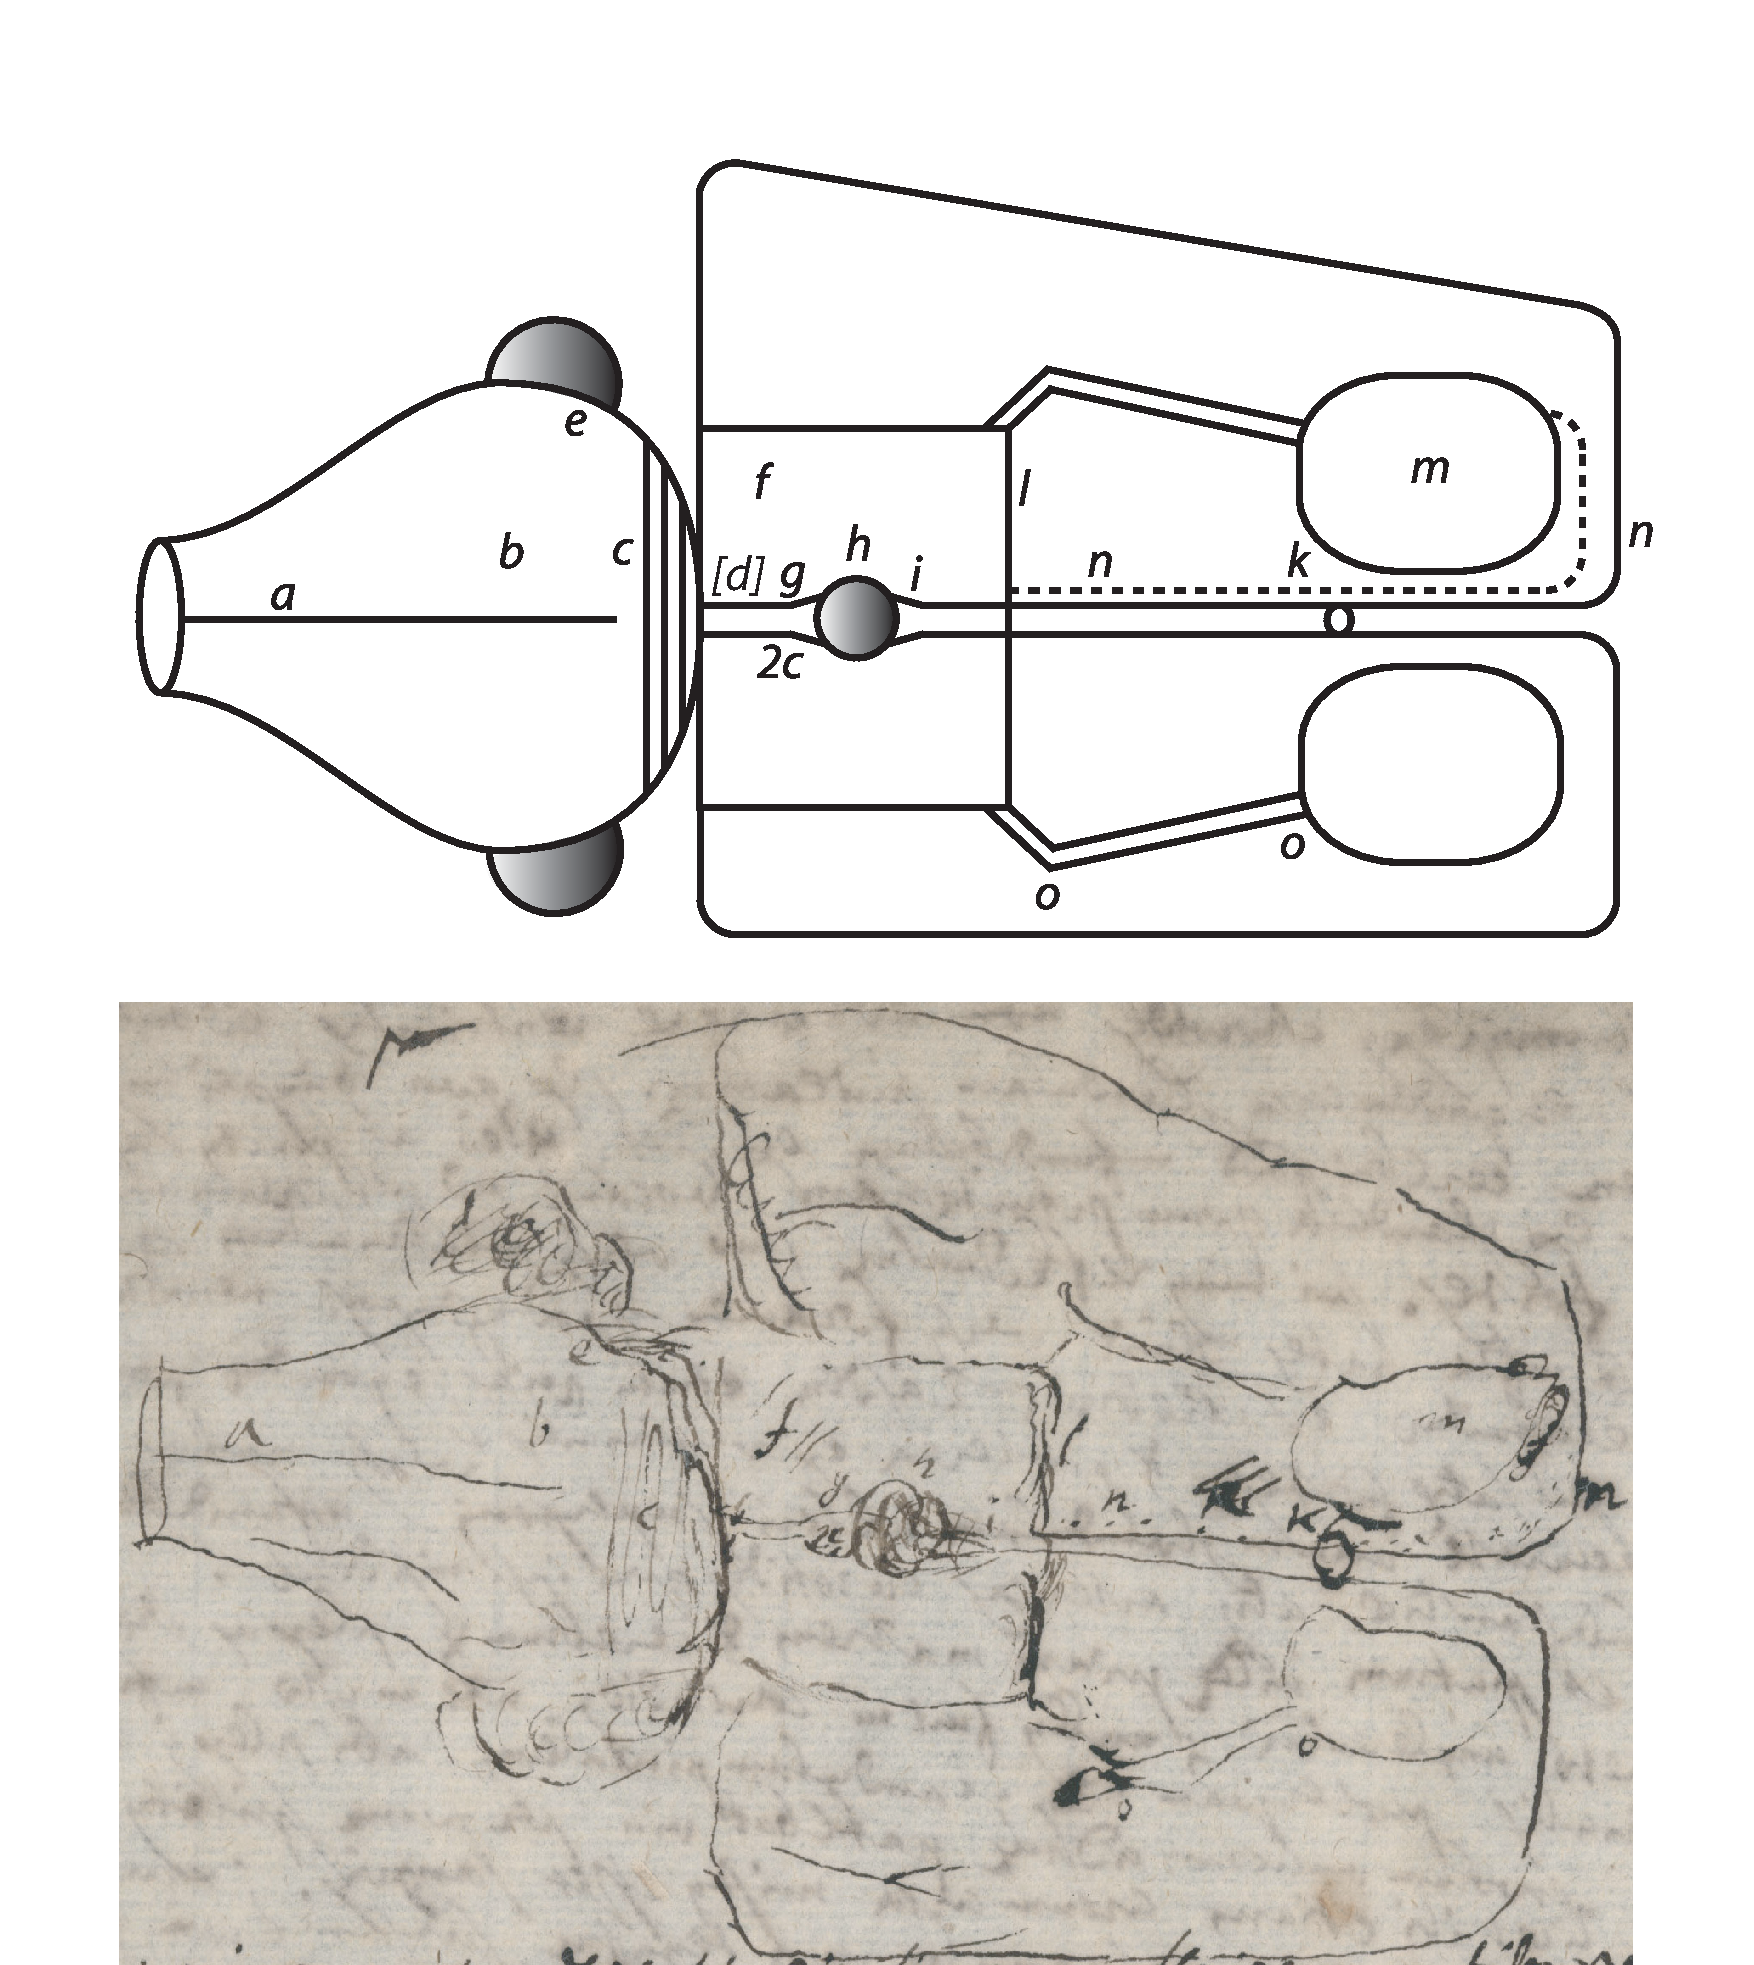
\includegraphics[width=0.75\textwidth]{images/lh0040104b_007r1.pdf}
%\newline%
%\rule[0mm]{0mm}{0mm}
%\lbrack\textit{Fig. 11}\rbrack
\pend
%\newpage% PR: Rein provisorisch !!!
\vspace{1.0em}% PR: Diesen leeren Zeilenabstand bitte behalten. Neuer Abschnitt !!!
\count\Bfootins=1200
\count\Cfootins=1200
\count\Afootins=1200
\pstart%
\noindent% Neuer Abschnitt.
\edtext{In}{\lemma{}\Afootnote{\textit{Am oberen Rand von Bl. 7~r\textsuperscript{o}:} Pars III. Excerptorum Anatomicorum ex Ms. Cartesii\protect\index{Namensregister}{\textso{Descartes}, Ren\'{e} (1596-1650)}}} ovis cerebro primo animadverti ejus figuram inferiorem partibus parum laxatis ut melius distingueretur circiter talem esse, $ab$ spinalis medulla; $c$ processus quem pontem cerebelli nominant, $d$ cerebellum; $e$ nervus 5\textsuperscript{ti} paris; $f$ nervus quarti paris, ex $g$ ad $h$ cavitas exigua, supra quam eminet quasi colliculus $h$ quem sequitur vallis versus $i$ ibique est foramen quod vulvam vocant, et ad $l$ est concursus nervorum opticorum vulvae rimam terminans; ibique exterius spinalis medulla terminatur. $k$ est protuberantia alba, quae separatis aliquantulum cerebri duabus partibus apparet easque unit; $m$ est processus
\edtext{mamillaris; $n$ punctu est nigricans}{%
\lemma{mamillaris;}\Bfootnote{%
\textit{(1)}\ $n$ pun %
\textit{(2)}\ $n$ %
\textit{(3)}\ $n$ \textbar\ punctu est \textit{erg.} \textbar\ nigricans \textit{L}}}
color intra processus mamillares in cerebri superficie conspicuus: in cavitate ad $h$ nullum vidi foramen; postquam cerebrum in aqua pernoctasset notavi nervorum opticorum substantiam esse mollissimam, contra aliorum omnium durissimam; quatenus extra medullam spinalem egrediebantur; in ipsa autem medulla radices nullas habere duriores. Pia mater erat etiam longe durior, quam prius.
\pend
\newpage
%\vspace{2em}
\pstart
\centering
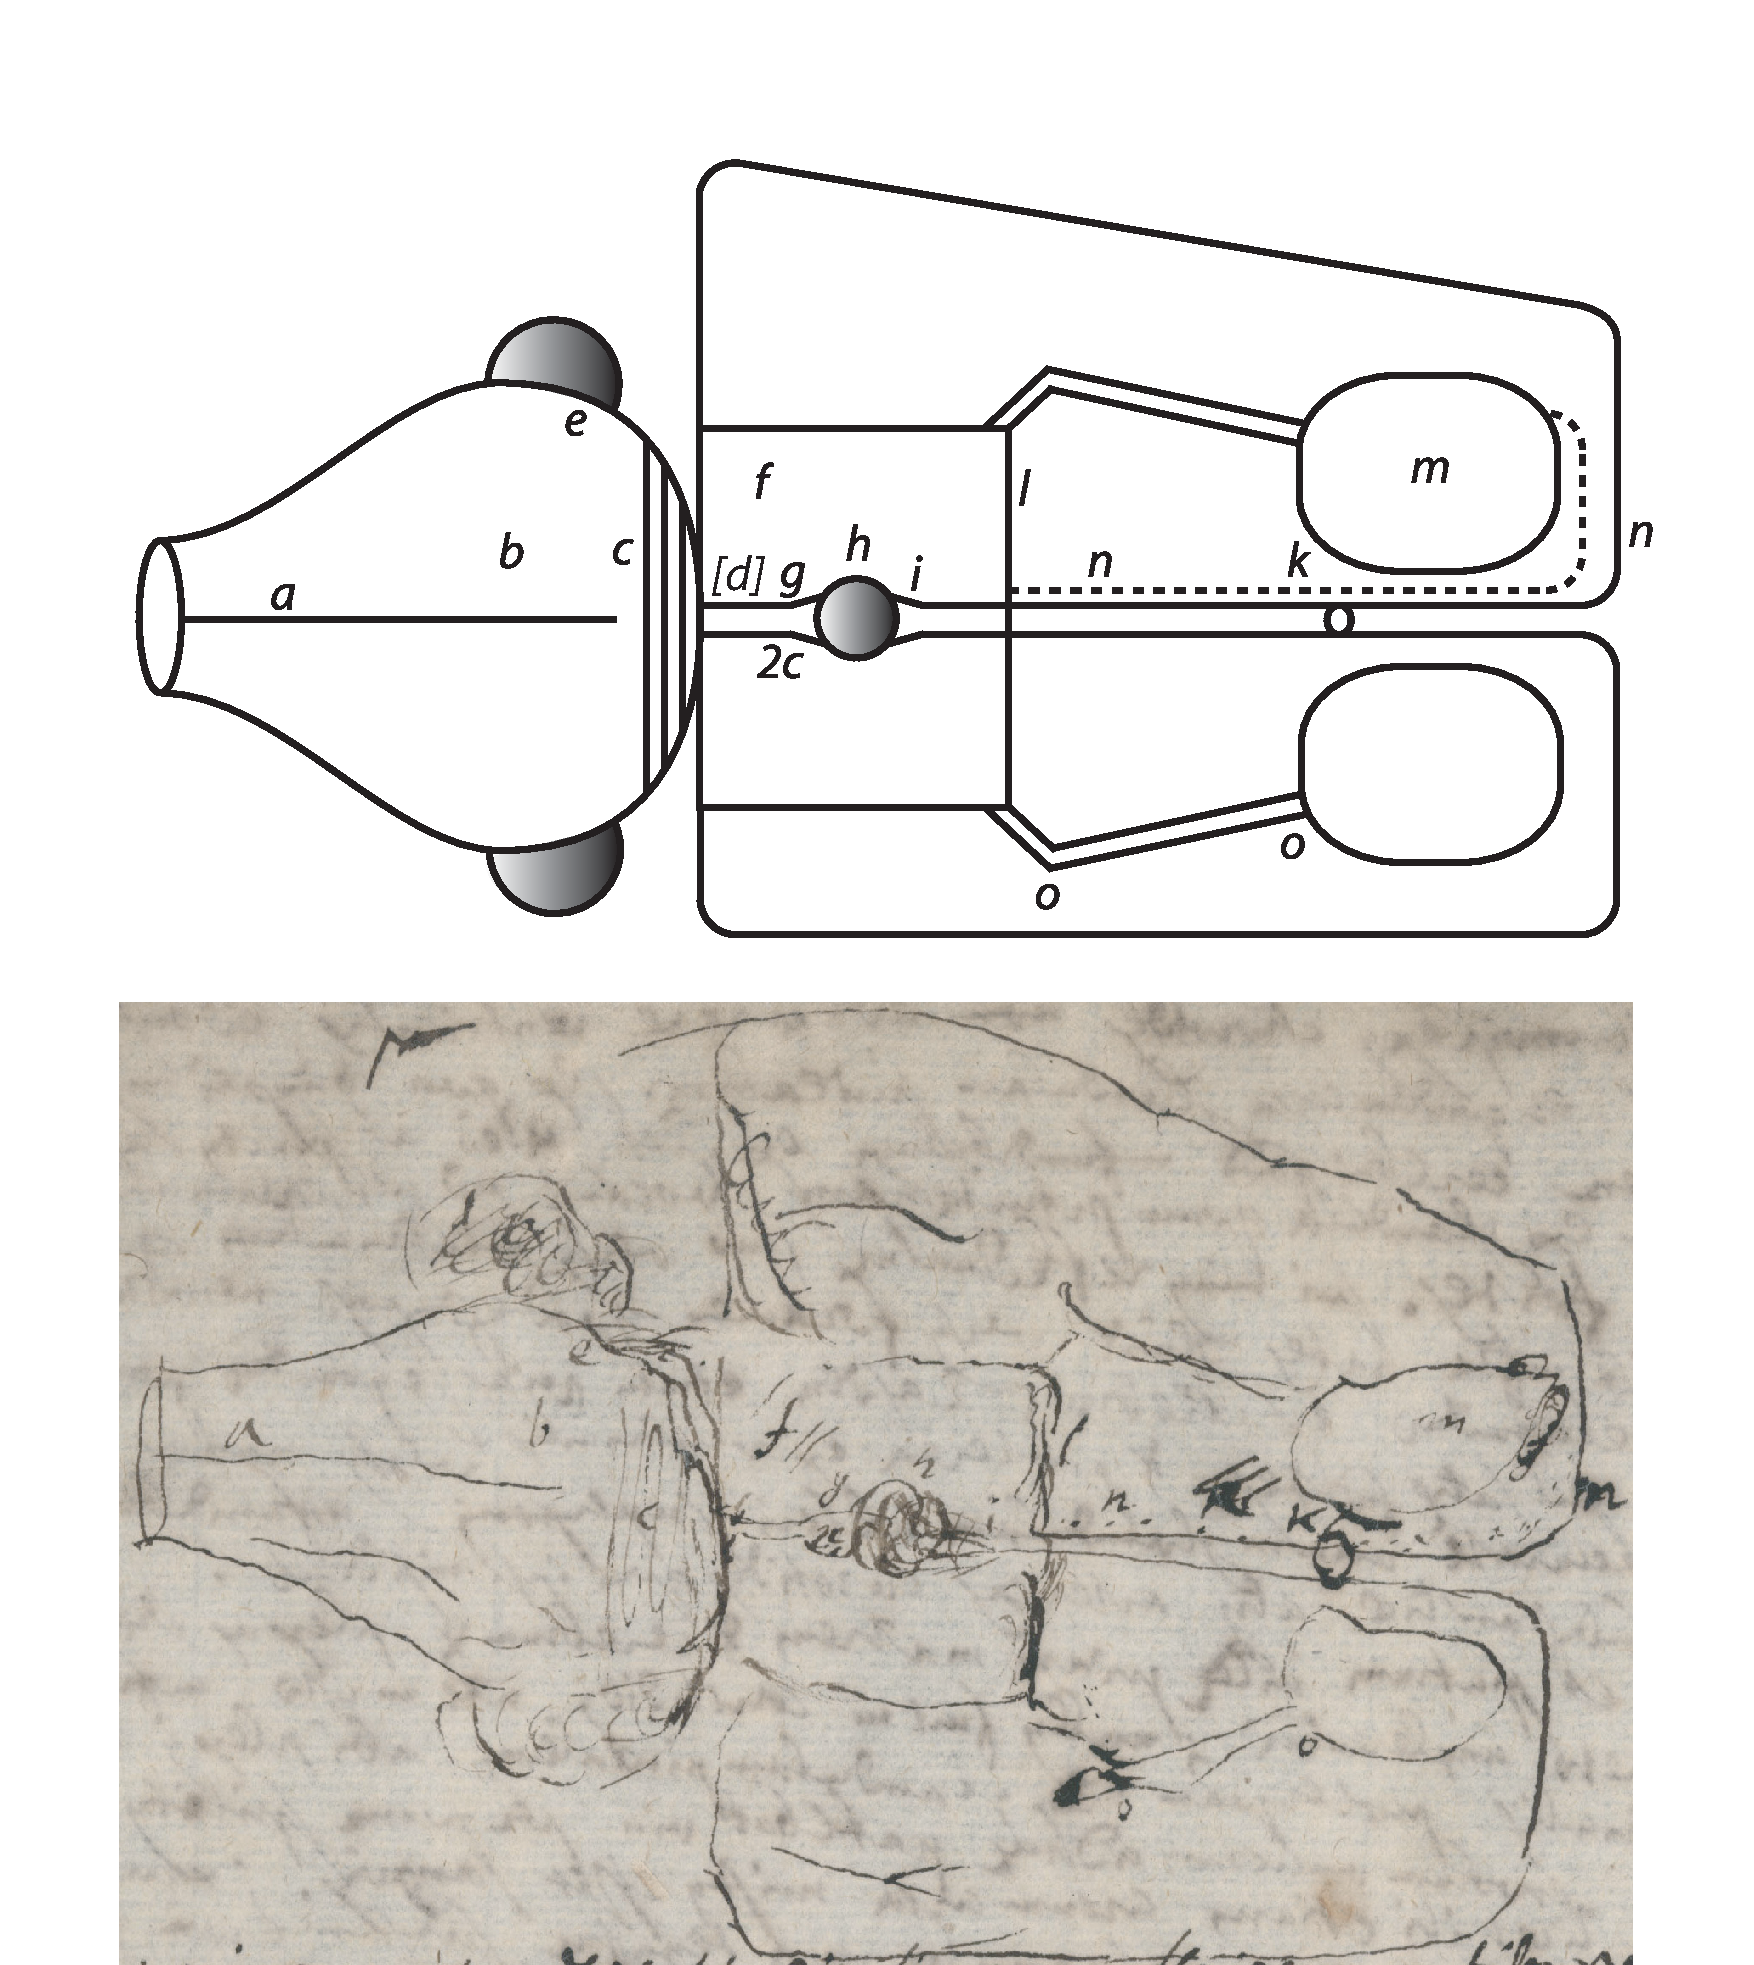
\includegraphics[trim = 0mm -5mm 0mm 0mm, clip, width=0.95\textwidth]{images/lh0040104b_007r1.pdf}\\
\centering \lbrack\textit{Fig. 11}\rbrack
\pend
\newpage
%\vspace{1em}
\pstart%
\centering
 \includegraphics[trim = 0mm 0mm 0mm 0mm, clip, width=0.4\textwidth]{images/lh0040104b_007r2.pdf}\\
\centering \lbrack\textit{Fig. 12}\rbrack
%\caption{Bildbeschreibung}
\pend
\vspace{1.5em}
\pstart
Inverso \setline{1}cerebro, notavi superius torcular Lambda efficere intra duas partes cerebri et cerebellum,
et emittere vas insigne e medio versus pelvim ejusque partem reflecti supra fornicem qui fornix incipit supra tertiam plicam medullae
\edtext{spinalis; cerebelli}{\lemma{spinalis;}\Bfootnote{\textit{(1)}\ cerebri parte \textit{(2)}\ cerebelli \textit{ L}}}
fibrae in medio erant transversae et fere etiam ad latera
\edtext{cerebri erant}{\lemma{}\Bfootnote{cerebri \textbar\ etiam \textit{gestr.}\ \textbar\ erant \textit{L}}} potius oblongae.
Medulla cerebelli una cum
\edtext{ejus ponte,}{\lemma{ejus}\Bfootnote{\textit{(1)}\ parte \textit{(2)}\ ponte, \textit{L}}}
qui totus etiam est ex medulla videtur \edtext{crassum annulum}{\lemma{crassum}\Bfootnote{\textit{(1)}\ annullu \textit{(2)}\ annulum \textit{L}}}
efficere, totam medullam spinalem ambientem.
Sed illi adhaeret inseparabiliter hic annulus ubique praeterquam sursum, ubi spinalis medulla est excavata et processus vermiformis deorsum reflectitur,
ut illam cavitatem impleat, estque haec cavitas cerebelli ventriculus.
Hanc cavitatem sequitur foramen infra 4\textsuperscript{am} plicam,
sive protuberantiam spinalis medullae, quae omnium minima est,
nec ejus duo latera rima distinguuntur ut aliae, sed linea recta,
quae est unum ex vinculis duorum laterum spinalis medullae.
$a$ podex $bb$ vinculum hoc ubi $b$ est 4\textsuperscript{a} plica interior spinalis medullae;
atque haec 4\textsuperscript{ta} plica directe occurrit intra cerebrum et cerebellum,
ideoque nulla rima secundas ejus partes separat,
quod nulla excrementa illac debent transire sed tertia plica quae proprie natibus potest assimilari rimam habet intermediam;
subjacet enim posteriori parti cerebri, ex qua nonulla excrementa in pelvem delabi
\edtext{possunt. Hac}{\lemma{possunt.}\Bfootnote{\textit{(1)}\ Hoc \textit{(2)}\ Hac \textit{L}}}
autem 3\textsuperscript{a} plica videntur duo tuberculi subrubri superstantes supra tabulatum album
cujus una pars est $bb,$ $dd$ altera; $cc$ sunt duo tubercula, $e$ est penis obturans foramen
per quod ex ventriculis cerebri delabuntur excrementa in pelvim.
Huic ad foramen quod podicem vocavi continuus est canalis rectus ab $a$ ad pelvim $e$ cui superstat planum $ae$ album;
denique infra $e.$
Inter $e$ et $f$ duae partes secundae plicae inter se uniuntur, ita ut excrementa partium anteriorum per $f$ possint labi in pelvim et illa posteriorum per $e.$
\pend%
\pstart%
In aure ovis ossicula tria sunt, sed
\edtext{paulo minora}{\lemma{paulo}\Bfootnote{\textit{(1)}\ majora \textit{(2)}\ minora \textit{L}}}
quam in vitulis excepto malleo, qui proportione major est.
Stapes \edtext{[auris]}{\lemma{cum}\Bfootnote{\textit{L \"{a}ndert Hrsg.}}}
utriusque est plane ejusdem figurae %\rule[-4mm]{0mm}{10mm}
\includegraphics[trim = 0mm 1mm 0mm 0mm, clip,width=0.1\textwidth]{images/lh0040104b_007r3.pdf} incumbitque supra membranulam claudentem unam ex fenestellis cochleae et labyrintho communibus. Nervi auditorii notavi tres ramos praeter partem duram, quae per proprium canalem ferebatur: praecipuus ramus directe ferebatur ad medium orbium cochleae; 2\textsuperscript{dus} multo minor directe infra stapedem, ubi incipiebat canalis ter revolutus labirinthi, 3\textsuperscript{us} rursus in labirintho inter primam et secundam
\edtext{revolutionem canalis,}{\lemma{revolutionem}\Bfootnote{\textit{(1)}\ cochleae; \textit{(2)}\ canalis, \textit{L}}}
cujus 1\textsuperscript{ma} revolutio tantae erat magnitudinis \rule[-2.5mm]{0mm}{12.5mm}\includegraphics[width=0.2\textwidth]{images/lh0040104b_007r4.pdf} vel \includegraphics[width=0.2\textwidth]{images/lh0040104b_007r5.pdf} et figurae \rule[-2mm]{0mm}{10mm}\includegraphics[width=0.2\textwidth]{images/lh0040104b_007r6.pdf} cochlea est \includegraphics[width=0.2\textwidth]{images/lh0040104b_007r7.pdf} canalis spiralis sensim in angustam desinens, vel potius duo canales conjuncti, videturque patere tantum ingressum ex fenestella ovali in initium unius ex istis canalibus, sed ex ejus fine rursum patere ingressum in finem sive angustiorem extremitatem alterius canalis;
et denique ex altera latiore extremitate hujus secundi canalis via quaedam patet extra os petrosum ut videtur, versus cerebrum, an vacua sit ista via, vel nervus, vel aliud quid illam impleat, nondum scio.
[7~v\textsuperscript{o}]%
\pend%
%\count\Bfootins=1500
%\count\Cfootins=1500
%\count\Afootins=1500